\chapter{Empirical Risk Minimisation}
We want an hypothesis$h \in H  h:X\rightarrow Y $ such that $h(x) \approx y$ for \textbf{any} data point $ (x,y)$, any datapoint means according to the distribution.
We want interpret the data point as realizations of i.i.d. random variables with probability distribution p(x,y) because the datapoint are part of the entire dataset. Define loss incurred for any data point as the expected loss, i.e., on average what will be the loss on the points of the distribution. Also called as \textbf{expected risk} or \textbf{Bayes risk}:
\begin{center}
    $E\{L((x,y),h)\} := \int_{x,y} L((x,y),h) d p (x,y) $
\end{center}
It is our integral weighted by the probability distribution. So to compute this expectation we need to know the probability distribution p(x,y) of data points (x,y).

However our goal is take the best hypothesis $h$ from the space of $H$ to minimize the expected loss, but estimate p(x,y) can be really difficult and not accurate, so the idea is approximate expected loss by average loss on data points (training set) called \textbf{empirical risk }.
\begin{center}
   Starting from Data $D = {(x^{(1)} , y^{(1)}), \dots , (x^{(m)} , y^{(m)})}$ with our m samples.\\
   We use that samples to compute the loss on the m samples $ \hat{L}(h|D) = \frac{1}{m} \sum\limits_{i=1}^m L((x^{(i)}, y^{(i)} ),h)$\\
   because for sufficiently larger (enough) sample size m $E\{L((x,y),h)\} \approx \Hat{L}(h|D) $\\
  \textbf{ \textit{learn hypothesis out of a hypothesis space or model that incurs minimum average loss when predicting labels of training datapoints based on their features}}
\end{center}
\begin{figure}[H]
    \centering
    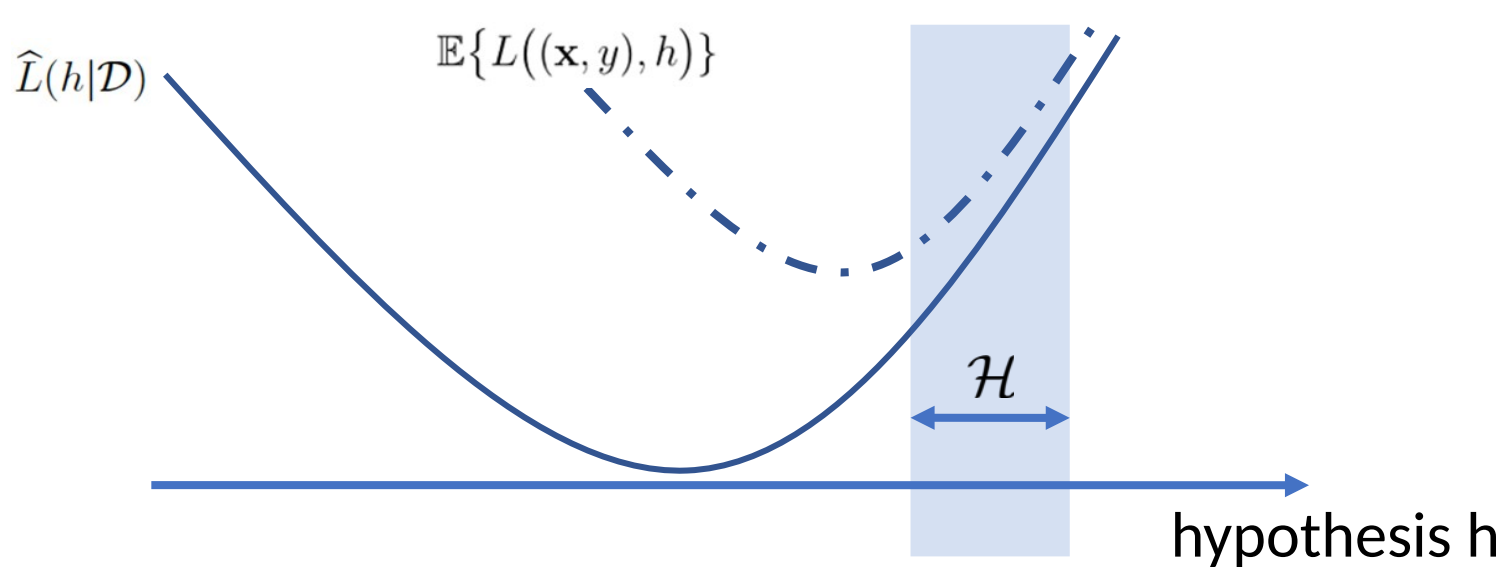
\includegraphics[scale=0.3]{images/ERM/ERM1.png}
    \caption{Empirical risk minimization}
    \label{fig:enter-label}
\end{figure}
In the picture above we have the 2 function of expected loss ($E$) and empirical loss ($L$) and our hypothesis $h$, but we have to consider only the $H$ space in light blue so the minimization of the 2 two function are equal in the left limit of $H$ that for both functions is closer to $h$.

If we have a parameterized function instead of considering the hypothesis space, so finding the best parameters instead of the best function we can transform $ h \in H \rightarrow w \in \mathbb{R}^n$.
\begin{center}
    With this change we can learnt parameters vector $\hat{w} = argmin f(w)$ with $ w\in \mathbb{R}^n$\\
  $  f(w) := \dfrac{1}{m} \sum\limits_{i=1}^m  L((x^{(i)}, y^{(i)} ),h^{(w)}) \rightarrow \hat{L} (h^{(w)} | \mathbb{D}) $ 
\end{center}
\begin{figure}[H]
    \centering
    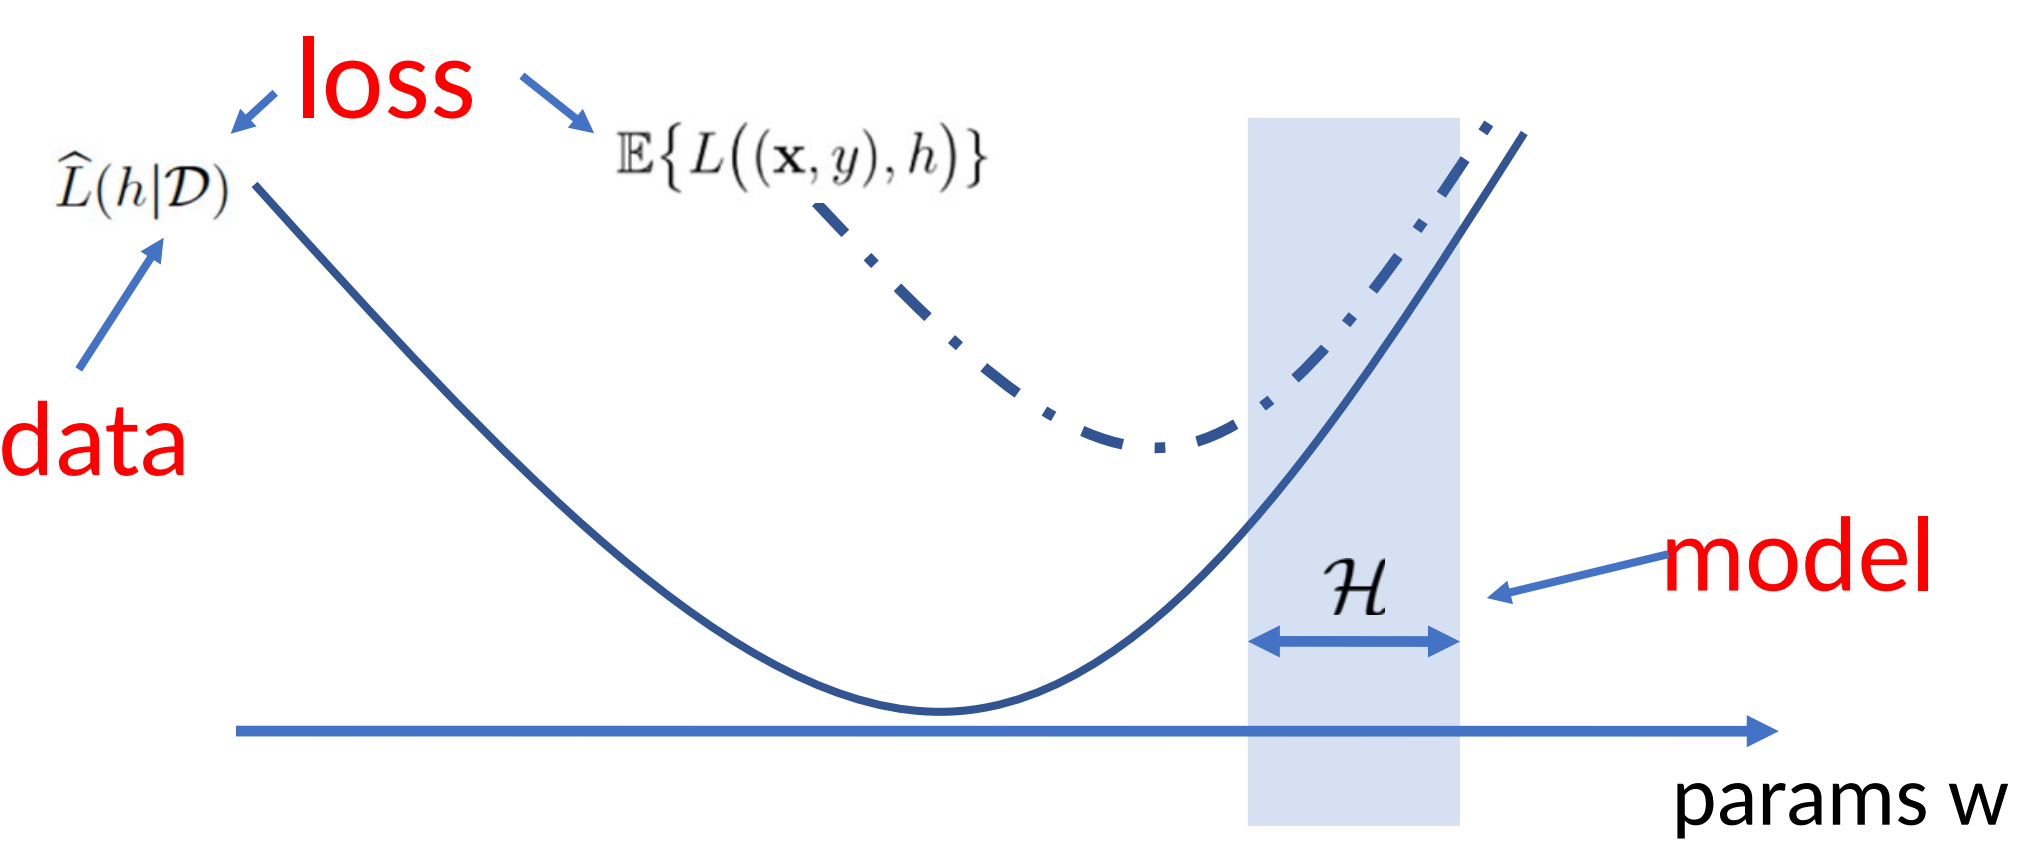
\includegraphics[scale=0.15]{images/ERM/ERM2.png}
    \caption{Design choices in erm}
    \label{fig:enter-label}
\end{figure}
 After all that assumption we can rewrite the machine learning definition :Learn a hypothesis in model that incurs in smallest empirical risk (loss) when predicting labels of training data points.
\section{Regression}
In any type of regression we have to define Data Model and loss, obviously in a regression the data can only have numeric type.

The formula has to work on the weights to apply on the n features that we have so the generic formula for the weights is: $ h^{(w)} (x) = w^T x= w_1 x_1+ \dots + w_n x_n$.\\
This is done to choose parameter/weight vector w to minimize average squared error loss or other error loss.\\
The example for linear regression became: $ \hat{w}= argmin (1/m) \sum\limits_{i=1}^i (j^{(i)} - w^T x^(i))^2 $
\begin{figure}[H]
    \centering
    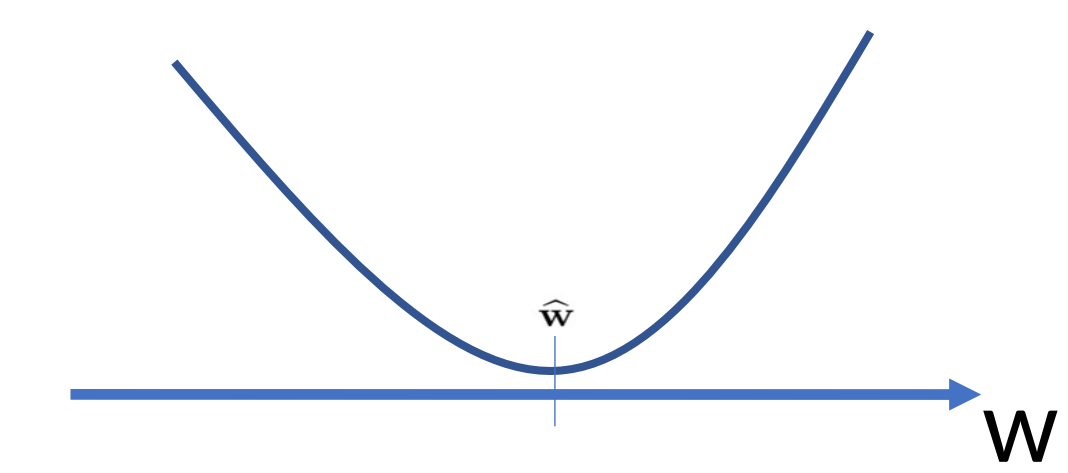
\includegraphics[scale=0.25]{images/ERM/ERm3.png}
    \caption{Example of linear regression with $\hat{w}$}
    \label{fig:enter-label}
\end{figure}

The feature map is a strategy that, starting from one single feature we create n feature applying different formulas to the single one, and than the process is the same to create a polynomial regression with different power up to the number of created features, creating bigger model with more flexibility:\\
$\mathbf{H}^{(n)}_{poly} = \{ h^{(w)}: \mathbb{R} \rightarrow \mathbb{R} : h^{(w)} (x) = \sum\limits_{j=1}^n x_j x^{j-1}$ with some $w = (w_1, \dots, x_n)^T \in \mathbb{R}^n  \} $
\begin{figure}[H]
    \centering
    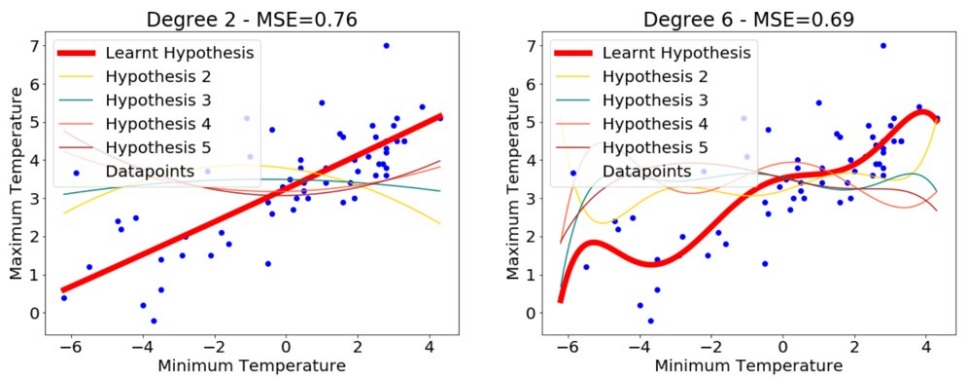
\includegraphics[scale=0.4]{images/ERM/ERM4.png}
    \caption{Comparison between degree}
    \label{fig:enter-label}
\end{figure}

There are different type pf calculating the error and we will see, as we already seen, the absolute, squared and a new one called Huber.

\begin{table}
    \centering
    \begin{tabular}{cccc}
         & Differentiable & Robust to outlier & Insensitive to noise \\
        Absolute loss & No & Yes & No\\
        Squared loss & Yes & No & Yes\\
        Huber loss & Yes & Yes & Yes\\
    \end{tabular}
    \caption{Caption}
    \label{tab:my_label}
\end{table}

All of them are convex function, but Huber loss merge them to use squared error loss when we are closer then $\epsilon$ and absolute error loss when we are further. Moreover this permit to don't depend on the outlier but have a more stable error function. The loss function have to be convex, because are simpler to minimize e differentiable for the same reason.
\begin{equation}
   L((x,y), h) =
    \begin{cases}
     (1/2)(y-h(x))^2 & for |y-h(x)| \ge \epsilon \\
     \epsilon (| y-h(x)| - \epsilon/2)\ & else
    \end{cases}       
\end{equation}

\section{Classification}

In classification we don't have number so we can't use the distance or function in same space, we have to obtain them through confidence measures. The output will be a label or multi-label.

Data points with numeric features, same as in linear regression. Model = space of linear maps, same as in linear regression; the change is in Logistic loss that is different from linear regression.

We need a formula that changes according to the output as $ L((x,y) ,h) := log (1+exp (-yh(x))) $, with squared error loss we can't because we aren't change between the two part (less and more than 0 ) of the function.

\begin{figure}[H]
    \centering
    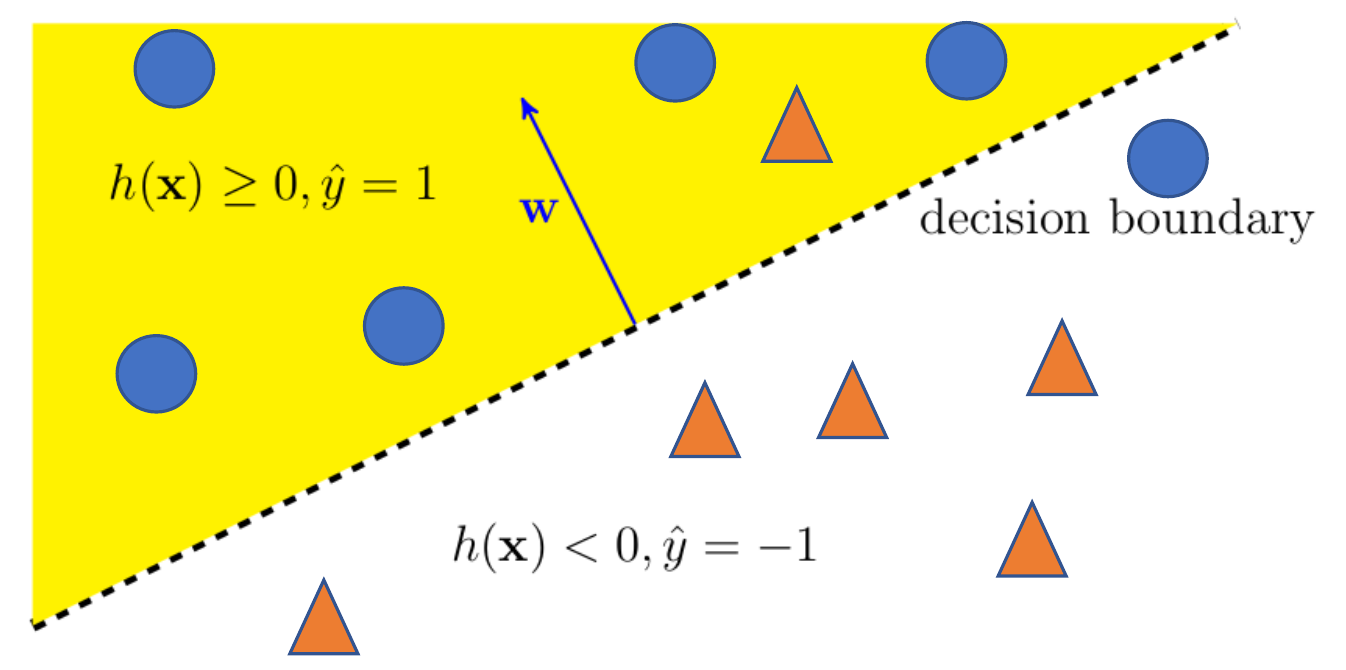
\includegraphics[scale=0.3]{images/ERM/ERM5.png}
    \caption{Logistic regression}
    \label{fig:enter-label}
\end{figure}


\paragraph{Losses in classification:}: the 0/1 loss isn't differentiable and non convex, 
\begin{equation}
   L((x,y), h) =
    \begin{cases}
     1 & for y \ne \hat{y} \\
     0 & else
    \end{cases}       
\end{equation}

Hinge loss $L((x,y), h) := max \{ 0,1 - yh(x) \}$, it is convex but non differentiable

\begin{figure}[H]
    \centering
    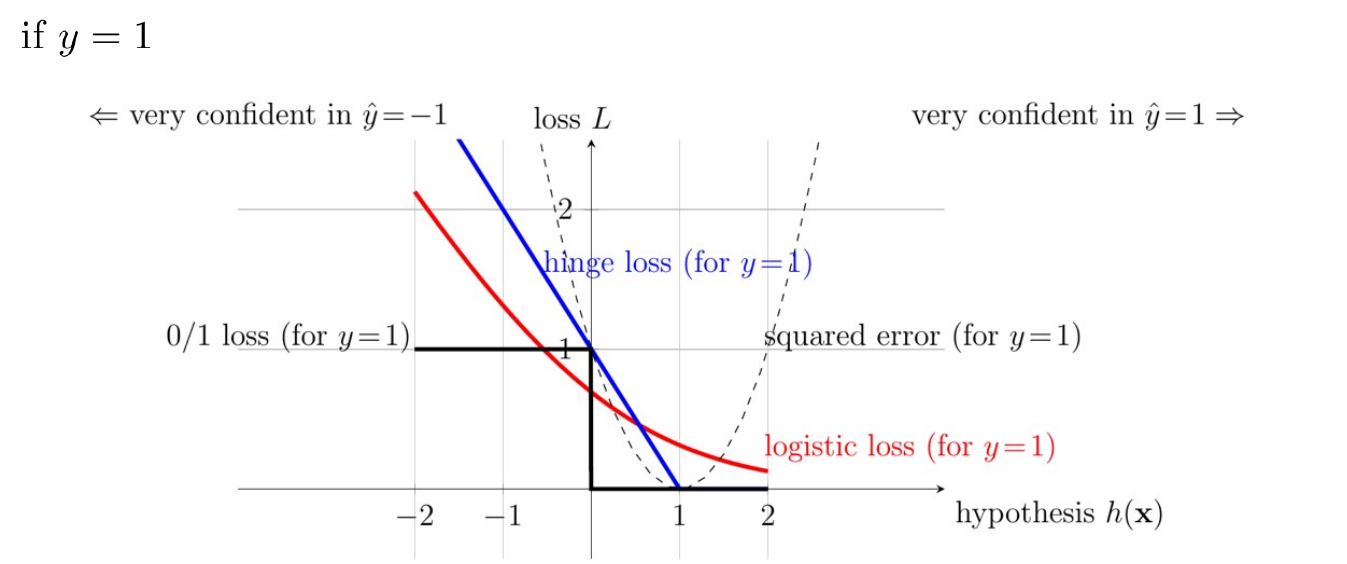
\includegraphics[scale=0.4]{images/ERM/ERM6.png}
    \caption{Comparison between losses}
    \label{fig:enter-label}
\end{figure}